%!TEX root = ../bare_jrnl.tex

\section{The Partially Observable Poisson Process}
\label{sec:popp}

The \emph{partially observable} Poisson process (POPP) is a counting process $N(t)$ with arrival rate $\lambda$ where the number of events appearing over the time interval $[0, t)$ is observed by one or more \emph{unreliable} counters. 
% 
The definition brings a distinction between the \emph{true count} (or simply \emph{count}), which refers to the number of events that actually occurred, and the \emph{sensed count}, which refers to the count obtained by a counter (or sensor). Let $c_i$ represent the true count over the interval $[0, t)$ during the $i$-th observation. With $m$ counters unreliably observing $c_i$, we use  $s_{j,i}$ to represent the sensed count given by sensor $j$ in the $i$-th observation within the interval $[0, t)$ with $1 \leq j \leq m$. Let $\mathbf{s_i} = (s_{1,i}, \ldots, s_{m,i})$ represent a vector of sensed counts from $m$ sensors for the $i$-th observation of the process. 

\begin{figure}[t!]
	\centering
%	\begin{tikzpicture}
%	\tikzstyle{place}=[circle,draw=blue,thick,minimum size=15 mm]
%	\tikzstyle{small}=[circle,draw=blue,thick,minimum size=8 mm]
%	\tikzstyle{every label}=[black]
%	\begin{scope}
%	\node[place](31)[xshift=0mm]{$\lambda$};
%	\node[place](21)[below of=31, yshift=-10mm]{$c_i$} edge[pre](31);
%	\node[small](11)[below of=21, yshift=-10mm]{$\ldots$} edge[pre](21);
%	\node[place](12)[left of=11, xshift=-5mm]{$s_{2,i}$} edge[pre](21);
%	\node[place](13)[left of=12, xshift=-10mm]{$s_{1,i}$} edge[pre](21);
%	\node[place](14)[right of=11, xshift=5mm]{$s_{(m-1),i}$} edge[pre](21);
%	\node[place](15)[right of=14, xshift=10mm]{$s_{m,i}$} edge[pre](21);
%	\draw[thick]($(13.north west)+(-0.5,2.45)$) rectangle ($(15.south east)+(0.5,-0.5)$);
%	\end{scope}
%	\end{tikzpicture}
%    \digraph[scale=0.5]{abc}{
%    	
%    	subgraph cluster_1 {
%    		color=blue;
%    		ci[label="$c_{i}$"];
%    		s1i[label="$s_{1, i}$"];
%    		s2i[label="$s_{2, i}$"];
%    		dot[label="...", shape=plaintext];
%    		sm1i[label="$s_{(m-1), i}$"];
%    		smi[label="$s_{m, i}$"];
%    		ci -> s1i;
%    		ci -> s2i;
%    		ci -> dot;
%    		ci -> sm1i;
%    		ci -> smi;
%    	}
    	
%    	"$\lambda$" -> ci
%    }
    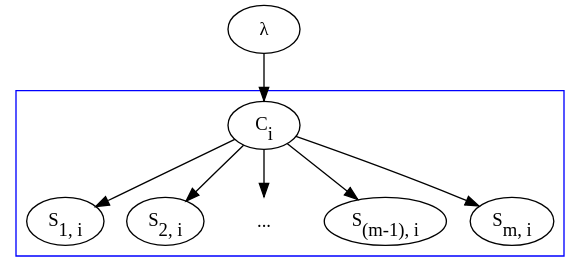
\includegraphics[width=0.5\textwidth]{./figures/gm_popp.png}
	\caption{Graphical representation of the partially observable Poisson process.}
	\label{fig:gm_popp}
\end{figure}
%\begin{figure}[t!]
%	\centering
%	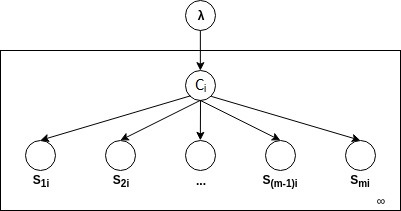
\includegraphics[width=0.5\textwidth]{./figures/gm_popp.jpg}
%    \caption{Graphical representation of the partially observable Poisson process.}
%	\label{fig:gm_popp}
%\end{figure}
Figure~\ref{fig:gm_popp} presents the graphical model derived from the definition of the POPP. This shows that the true count $c_i$ has become a latent variable which can only be inferred from the sensed count.
% 
The posterior of $\lambda$ is then inferred from the posterior of $c_i$ after $n$ observations, $i = 1 \ldots n$. 
% \textbf{TODO: Fix figure to have \emph{multiple} $c_i$s not a single $X_i$. \emph{$c_i$ can not be multiple since it is the true count at time interval $i$, the sensed count can be multiple since they may come from different sensors.}	}

% The rate parameter $\lambda$ of the POPP model can be inferred by marginalising over all possible true count values $c_i$ in $P(\lambda \mid c_i)$ and in the  distribution of true counts given sensed counts $P(c_i \mid \mathbf{s_i})$. 
The rate parameter $\lambda$ of the POPP model can be inferred by marginalising over all possible true count values $c_i$ and in the  distribution of true counts given sensed counts $P(c_i \mid \mathbf{s_i})$.
% 
Given $n$ observations of the underlying process, let all observed true counts be represented by $\mathbf{c} = (c_1, \ldots, c_n)$, and all sensed counts by $\mathbf{s}=(\mathbf{s_1} \dots \mathbf{s_n})$, for $1 \leq i \leq n$ (recalling each $\mathbf{s_n}$ is produced by $m$ sensors). 
% 
The posterior of $\lambda$ is then:
\begin{equation}
	\label{eq:marginal_occurrences}
	\begin{tabular}{r@{=}l}
		$P(\lambda \mid \mathbf{s})$ &  $\displaystyle\sum_{c_1=0}^{\infty} \ldots \displaystyle\sum_{c_n=0}^{\infty} P(\lambda \mid \mathbf{c}) ~ P(\mathbf{c} \mid \mathbf{s})$ \\
	\end{tabular}
\end{equation}
\noindent where true count probabilities, $P(\lambda \mid \mathbf{c})$, can be drawn from the original FOPP definition:
\begin{equation}
	\label{eq:gamma_posterior_fopp}
	\begin{tabular}{r@{ = }l}
		$P(\lambda \mid \mathbf{c})$ & $Gam\Bigg(\lambda \Bigm| \displaystyle\sum_{i=1}^{n} c_i + \alpha, n + \beta \Bigg)$
	\end{tabular}
\end{equation}
If we assume that the sensor counts for observation period $i$ are conditionally independent (i.e.~\textit{uncorrelated}) given the true count $c_i$, then the probability of a collection of observations given the true count is defined as follows: 
\begin{equation}
	\label{eq:independent_sensor_likelihood}
	\begin{tabular}{r@{=}l}
	$P(\mathbf{s_i} \mid c_i)$ & $\displaystyle\prod_{j=1}^{m} P(s_{j,i} \mid c_i)$ \\ 
	\end{tabular}
\end{equation}
Using this, the probability of a particular sequence of $n$ counts, given a sequence of $n$ observations each from $m$ sensors, $P(\mathbf{c} \mid \mathbf{s})$, can be defined as:
\begin{equation}
    \label{eq:occurrences_likelihood}
    \begin{tabular}{r@{ $\varpropto$ }l}
        $P(\mathbf{c} \mid \mathbf{s})$ & $P(\mathbf{s_1}, \ldots, \mathbf{s_n} \mid \mathbf{c}) ~ P(\mathbf{c})$ \\ [1ex]
        & $\displaystyle\prod_{i=1}^{n} P(\mathbf{s_i} \mid c_i) ~ P(c_i \mid \mathbf{s_{i-1}}, \ldots, \mathbf{s_{1}})$ \\ [2ex]
        & $\displaystyle\prod_{i=1}^{n} \displaystyle\prod_{j=1}^{m} P(s_{j,i} \mid c_i) ~ P(c_i \mid \mathbf{s_{-1}})$
    \end{tabular}
\end{equation}
\noindent where $\mathbf{s_{-1}} = \mathbf{s_{i-1}}, \ldots, \mathbf{s_1}$\footnote{$s_{-1}$ does not exist whenever $i = 1$, and \\ $P(c_i) = \int_{\lambda=0}^{\infty} P(c_i \mid \lambda) ~ Gam(\lambda \mid \alpha, \beta) ~d\lambda$} and \hspace{0.3cm}$P(c_i \mid \mathbf{s_{-1}})$ can be calculated as:
% $P(c_i \mid \mathbf{c_{-1}})$ can be calculated using a negative binomial distribution:
\begin{equation}
	\label{eq:unconditional_xi}
	\begin{tabular}{r@{=}l}
		$P(c_i \mid \mathbf{s_{-1}})$ & $\displaystyle\int_{\lambda=0}^{\infty} P(c_i \mid \lambda) ~ P(\lambda \mid \mathbf{s_{-1}}) ~d\lambda$ \\ [2ex]
		%& $\displaystyle\int_{\lambda=0}^{\infty} Poi(c_i \mid \lambda) ~ Gam(\lambda \mid \alpha_{-1}, \beta_{-1}) ~d\lambda$ \\ [2ex]
		%& $NB\Bigg(c_i \Bigm| \alpha_{-1}, \displaystyle\frac{\beta_{-1}}{\beta_{-1} + 1}\Bigg)$.
	\end{tabular}
\end{equation}
% \noindent with $P(\lambda \mid \mathbf{c_{-1}})$ that does not follow \ref{eq:gamma_posterior_fopp} since the hyperparameters $\alpha_{-1}, \beta_{-1}$ in $Gam(\lambda \mid \alpha_{-1}, \beta_{-1})$ are not the original hyperparameters $\alpha, \beta$ as in \ref{eq:gamma_posterior_fopp}. The hyperparameters $\alpha_{-1}, \beta_{-1}$ are the hyperparameters obtained after $P(\lambda \mid s_1, \ldots, s_{i-1})$ has been calculated.
To complete Eq. \ref{eq:occurrences_likelihood} we must also define $P(s_{j,i} \mid c_i)$. The Poisson limit theorem states that the Poisson distribution may be used as an approximation to the binomial distribution \cite{papoulis2002probability}. Using this theorem as the foundation, an arbitrarily close approximation to the probability $P(s_{j,i} \mid c_i)$ is defined by assuming there exists a small enough finite subinterval of length $\delta$ for which the probability of more than one event occurring is less than some small value $ \epsilon$ and that $\delta$ is small enough that $\epsilon$ is negligible. With this assumption, interval $[0, t)$ is split into $l$ smaller subintervals $I_1, \ldots, I_l$ of equal size, with the condition that $l > \lambda$. Consequently, the whole interval $[0, t) = I_1, \ldots, I_l$ becomes a series of Bernoulli trials, where the $k^{th}$ trial corresponds to whether (1) an event $e_k$ happens with probability $\lambda / l$ and (2) a sensor $j$ captures the event $e_k$ as the detection $d_k$ at the subinterval $I_k$.

Following this, $P(s_{j,i} \mid c_i)$ can be defined using of the count of true  positives given $c_i$ subintervals, and the false positives given the remaining $l-c_i$ subintervals. 
% 
Let the probability of a \textit{true positive detection} (TP) for sensor $j$ in a single subinterval be $\tau_j=P_j(d \mid e{=}1)$, and the probability of a \textit{false positive detection} (FP) be $\xi_j = P_j(d \mid e{=}0)$. Thus $P(s_{j,i} \mid c_i)$ is defined as a sum over all possible sensed counts of the product of two binomial distributions $B(r \mid n,\pi)$: 
\begin{equation}
	\label{eq:joint_binomial_distribution}
    P(s_{j,i} \mid c_i) \! = \! \! \! \displaystyle\sum_{r = 0}^{c_{i}} \! \! B\Big(r \mid c_i, \tau_j\Big) B\Big((s_{j,i} - r) \mid (l - c_{i}), \xi_j \Big)
\end{equation}
\noindent where the first binomial provides the probability of getting some proportion of the count from  TP detections and the second binomial provides the probability of getting the remainder from FP detections. 

% \textbf{NOTE: This constraints $s_{j,i} \leq c_i$, doesn't it? Is it worth commenting on this? If we don't want this then we need to introduce $l$ a little more formally than was done before. \emph{we do not constraint it, $s_{j, i}$ can be greater than $c_i$. if $s_{j, i}$ is greater than $c_i$ it means that some portion of $s_{j, i}$ contains false positive.}}

Eq.~\ref{eq:marginal_occurrences} shows the difficulty of estimation in the POPP model. Since no conjugate density provides an analytical solution for the posterior over $\lambda$, every sensed count $\mathbf{s_i}$ must be retained to calculate the posterior of $\lambda$. That means elements representing each value of $c_i$ on each observation grow infinitely. Even with an upper bound $l$ on the maximum value of $c_i$, the number of elements to retain on each observation periods grows exponentially.

% Therefore each of the $n$ observation periods adds a factor of a countably infinite number of elements, and therefore the posterior is a sum of countably infinite sums. Even with an upper bound $l$ on the maximum value of $c_i$, the number of elements in the posterior grows by $l$ with each observation period.
% 
\subsection*{$\lambda$ Estimators}\label{sec:estimators}

To address this difficulty, in~\cite{jovan18a} we proposed three estimators, each of which offers an approximation to the true posterior $P(\lambda \mid \mathbf{s})$. The estimators are: \\
(1) a \textit{gamma filter}, which approximates Eq.~\ref{eq:marginal_occurrences} with a single gamma distribution minimising the KL-divergence $D_{KL}(P(\lambda \mid \mathbf{s}) \mid \mid Gam(\lambda \mid \alpha, \beta))$ by gradient descent. The accuracy of this filter deteriorates as sensor reliability degrades. However, computation time is constant on each observation and Eq. \ref{eq:unconditional_xi} has a closed form, using the negative binomial distribution
\begin{equation}
\label{eq:unconditional_xi_gamma_filter}
\begin{tabular}{r@{=}l}
$P(c_i \mid \mathbf{s_{-1}})$ & $\displaystyle\int_{\lambda=0}^{\infty} P(c_i \mid \lambda) ~ P(\lambda \mid \mathbf{s_{-1}}) ~d\lambda$ \\ [2ex]
& $\displaystyle\int_{\lambda=0}^{\infty} Poi(c_i \mid \lambda) ~ Gam(\lambda \mid \alpha_{-1}, \beta_{-1}) ~d\lambda$ \\ [2ex]
& $NB\Bigg(c_i \Bigm| \alpha_{-1}, \displaystyle\frac{\beta_{-1}}{\beta_{-1} + 1}\Bigg)$.
\end{tabular}
\end{equation}
\noindent with the hyperparameters $\alpha_{-1}, \beta_{-1}$ in $Gam(\lambda \mid \alpha_{-1}, \beta_{-1})$ being the updated hyperparameters obtained after $P(\lambda \mid s_1, \ldots, s_{i-1})$ has been calculated;\\
(2) a \textit{histogram filter}, which approximates Eq.~\ref{eq:marginal_occurrences} with a discrete distribution $Q(\lambda \mid \mathbf{s})$ by quantising $\lambda$. The advantage of this filter over the gamma filter is that it can track the posterior to an arbitrary fidelity via a finer quantisation with the cost of computation time. Its disadvantage is an increase in computation time compared to the gamma filter; \\
(3) a \textit{switching filter}, which approximates Eq.~\ref{eq:marginal_occurrences} either by a gamma filter or by a histogram filter depending on whether $P(\lambda \mid \mathbf{s})$  resembles a gamma distribution and can be approximated by the gamma filter via KL-divergence $D_{KL}(P(\lambda \mid \mathbf{s}) \mid \mid Gam(\lambda \mid \alpha, \beta))$.

\begin{figure}[t!]
	\centering
	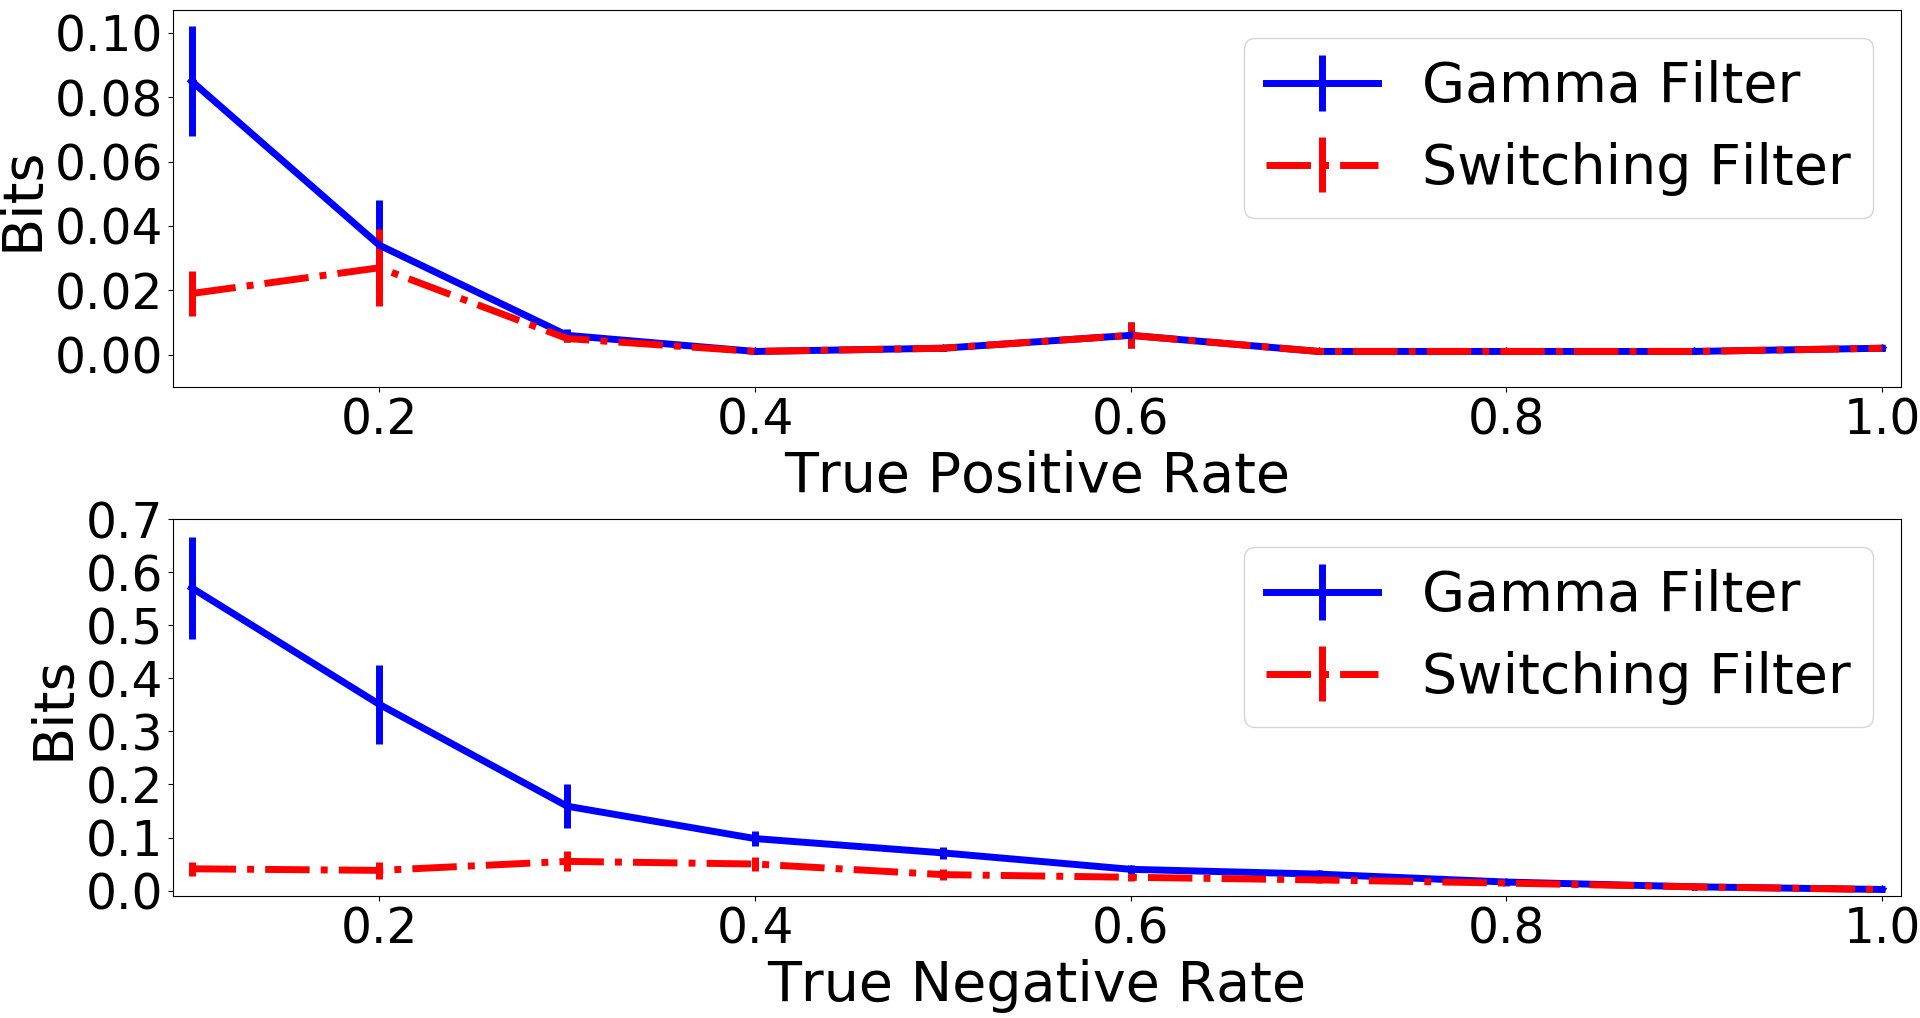
\includegraphics[width=0.5\textwidth]{./figures/kl_div_tpr_tnr_var.png}
	\caption{Average KL-divergence from the gamma and switching filters to $P(\lambda \mid \protect\mathbf{s})$. The horizontal axis shows the true positive rate (top) and true negative rate (bottom) of one simulated sensor. Standard error is shown.} 
	\label{fig:kl_div_tpr_tnr_var}
\end{figure}

In general (and in our experimental work from Section~\ref{sec:evasim} onwards) we use the switching filter as the estimator to the true posterior $P(\lambda \mid \mathbf{s})$ because it combines the best of both the gamma filter (fast calculation) and the histogram filter (accurate approximation) with minimum loss in similarity to the true posterior $P(\lambda \mid \mathbf{s})$. Figure \ref{fig:kl_div_tpr_tnr_var} shows KL-divergence between the gamma and switching filters to the true posterior over different sensor reliabilities using simulated data. Note that the histogram filter was not included because it perfectly tracked $P(\lambda \mid \mathbf{s})$, i.e., $D_{KL}(P(\lambda \mid \mathbf{s}) \mid \mid Q(\lambda \mid \mathbf{s})) \approx 0$. A more detailed presentation of these estimators is given in~\cite{jovan18a}.